
% JuliaCon proceedings template
\documentclass{juliacon}
\setcounter{page}{1}

\begin{document}

% **************GENERATED FILE, DO NOT EDIT**************

\title{BlankLocalizationCore.jl: implementing blank localization in Julia}

\author[1, 2]{Tamás Cserteg}
\author[1]{András Kovács}
\author[1, 3]{József Váncza}
\affil[1]{EPIC Centre of Excellence, HUN-REN Institute for Computer Science and Control (SZTAKI), Budapest H-1111, Hungary}
\affil[2]{Doctoral School of Informatics, ELTE Eötvös Loránd University, Budapest H-1117, Hungary}
\affil[3]{Department of Manufacturing Science and Technology, Budapest University of Technology and Economics, Budapest H-1111, Hungary}

\keywords{Julia, Optimization, Machining, Blank localization}

\hypersetup{
pdftitle = {BlankLocalizationCore.jl: implementing blank localization in Julia},
pdfsubject = {JuliaCon 2022 Proceedings},
pdfauthor = {Tamás Cserteg, András Kovács, József Váncza},
pdfkeywords = {Julia, Optimization, Machining, Blank localization},
}



\maketitle

\begin{abstract}

Blank localization (also known as workpiece referencing) is an essential task in machining.
It aims to precisely establish the geometric relation of the machine tool (mill, lathe, etc.) and the workpiece.
We introduced the concept of multi-operation blank localization to address this task for drilling and milling scenarios in a semi-automated way, which allows positioning different machining features (e.g., different holes) separately in order to exploit the tolerances on the relative position of those features to compensate the small errors of the blank.
The method takes as input the measured rough geometry and the machining CNC code, and computes the best possible position of each feature considering machining allowances and tolerances by solving a convex quadratically constrained quadratic program (QCQP).
The versatility and extensibility of the Julia language helped the development of this algorithm, materializing in the \texttt{BlankLocalizationCore.jl} package.
Its flexibility and ease of use make it an excellent research tool that can be deployed in production as well.
\end{abstract}

\section{Introduction}
\label{sec:intro}
Cast parts may have small geometric variations from lot to lot that need to be addressed before machining by altering the CNC code.
Current practice is dominated by iterative adjustments by the human operator, which requires highly trained workers, takes a long time, and still, may produce scrap.
Automated methods exist for complex free-form parts like wind turbines that place the entire blank as a single solid object (\cite{ding:2021_CoarsefineOptimizationMethod}\cite{tan:2014_UnconstrainedApproachBlank}).
Multi-operation blank localization was introduced in~\cite{cserteg:2023_Annals} focusing on drilling and milling.
These machining operations are among the most used ones, therefore the method is applicable for a wide range of products.
The abstract method and its implementation was developed in parallel, which required a language with support for easy prototyping and wide variety of tools.
Exactly for these reasons we chose the Julia language~\cite{bezanson2017julia}.

\section{Multi-operation blank localization}
\label{sec:algo}

The algorithm looks for the optimal position (part zero) for each feature group on the workpiece. 
Features within a group can be, for example, drilled holes on the same side of the part, whose drilling positions are defined relative to a common reference (the part zero).
Features within the same group must be moved together, but different feature groups can be moved separately.
The to-be-machined features (short: machined features) need to be aligned with the features on the blank (called rough features) in a way that a minimum machining allowance is ensured and the dimensional tolerances between features are respected.
The former encodes the requirement that material needs to be removed to ensure proper surface finish and is described for a feature as the smallest thickness of removed material.
A dimensional tolerance between two features is modeled as lower and upper bounds on the distance between the two features.
As feature groups move together, only inter-group tolerances need to be considered.
Fig.~\ref{fig:hatfig} shows two feature groups with their part zeros, as well as the tolerances between features.

\begin{figure}[b]
	\centerline{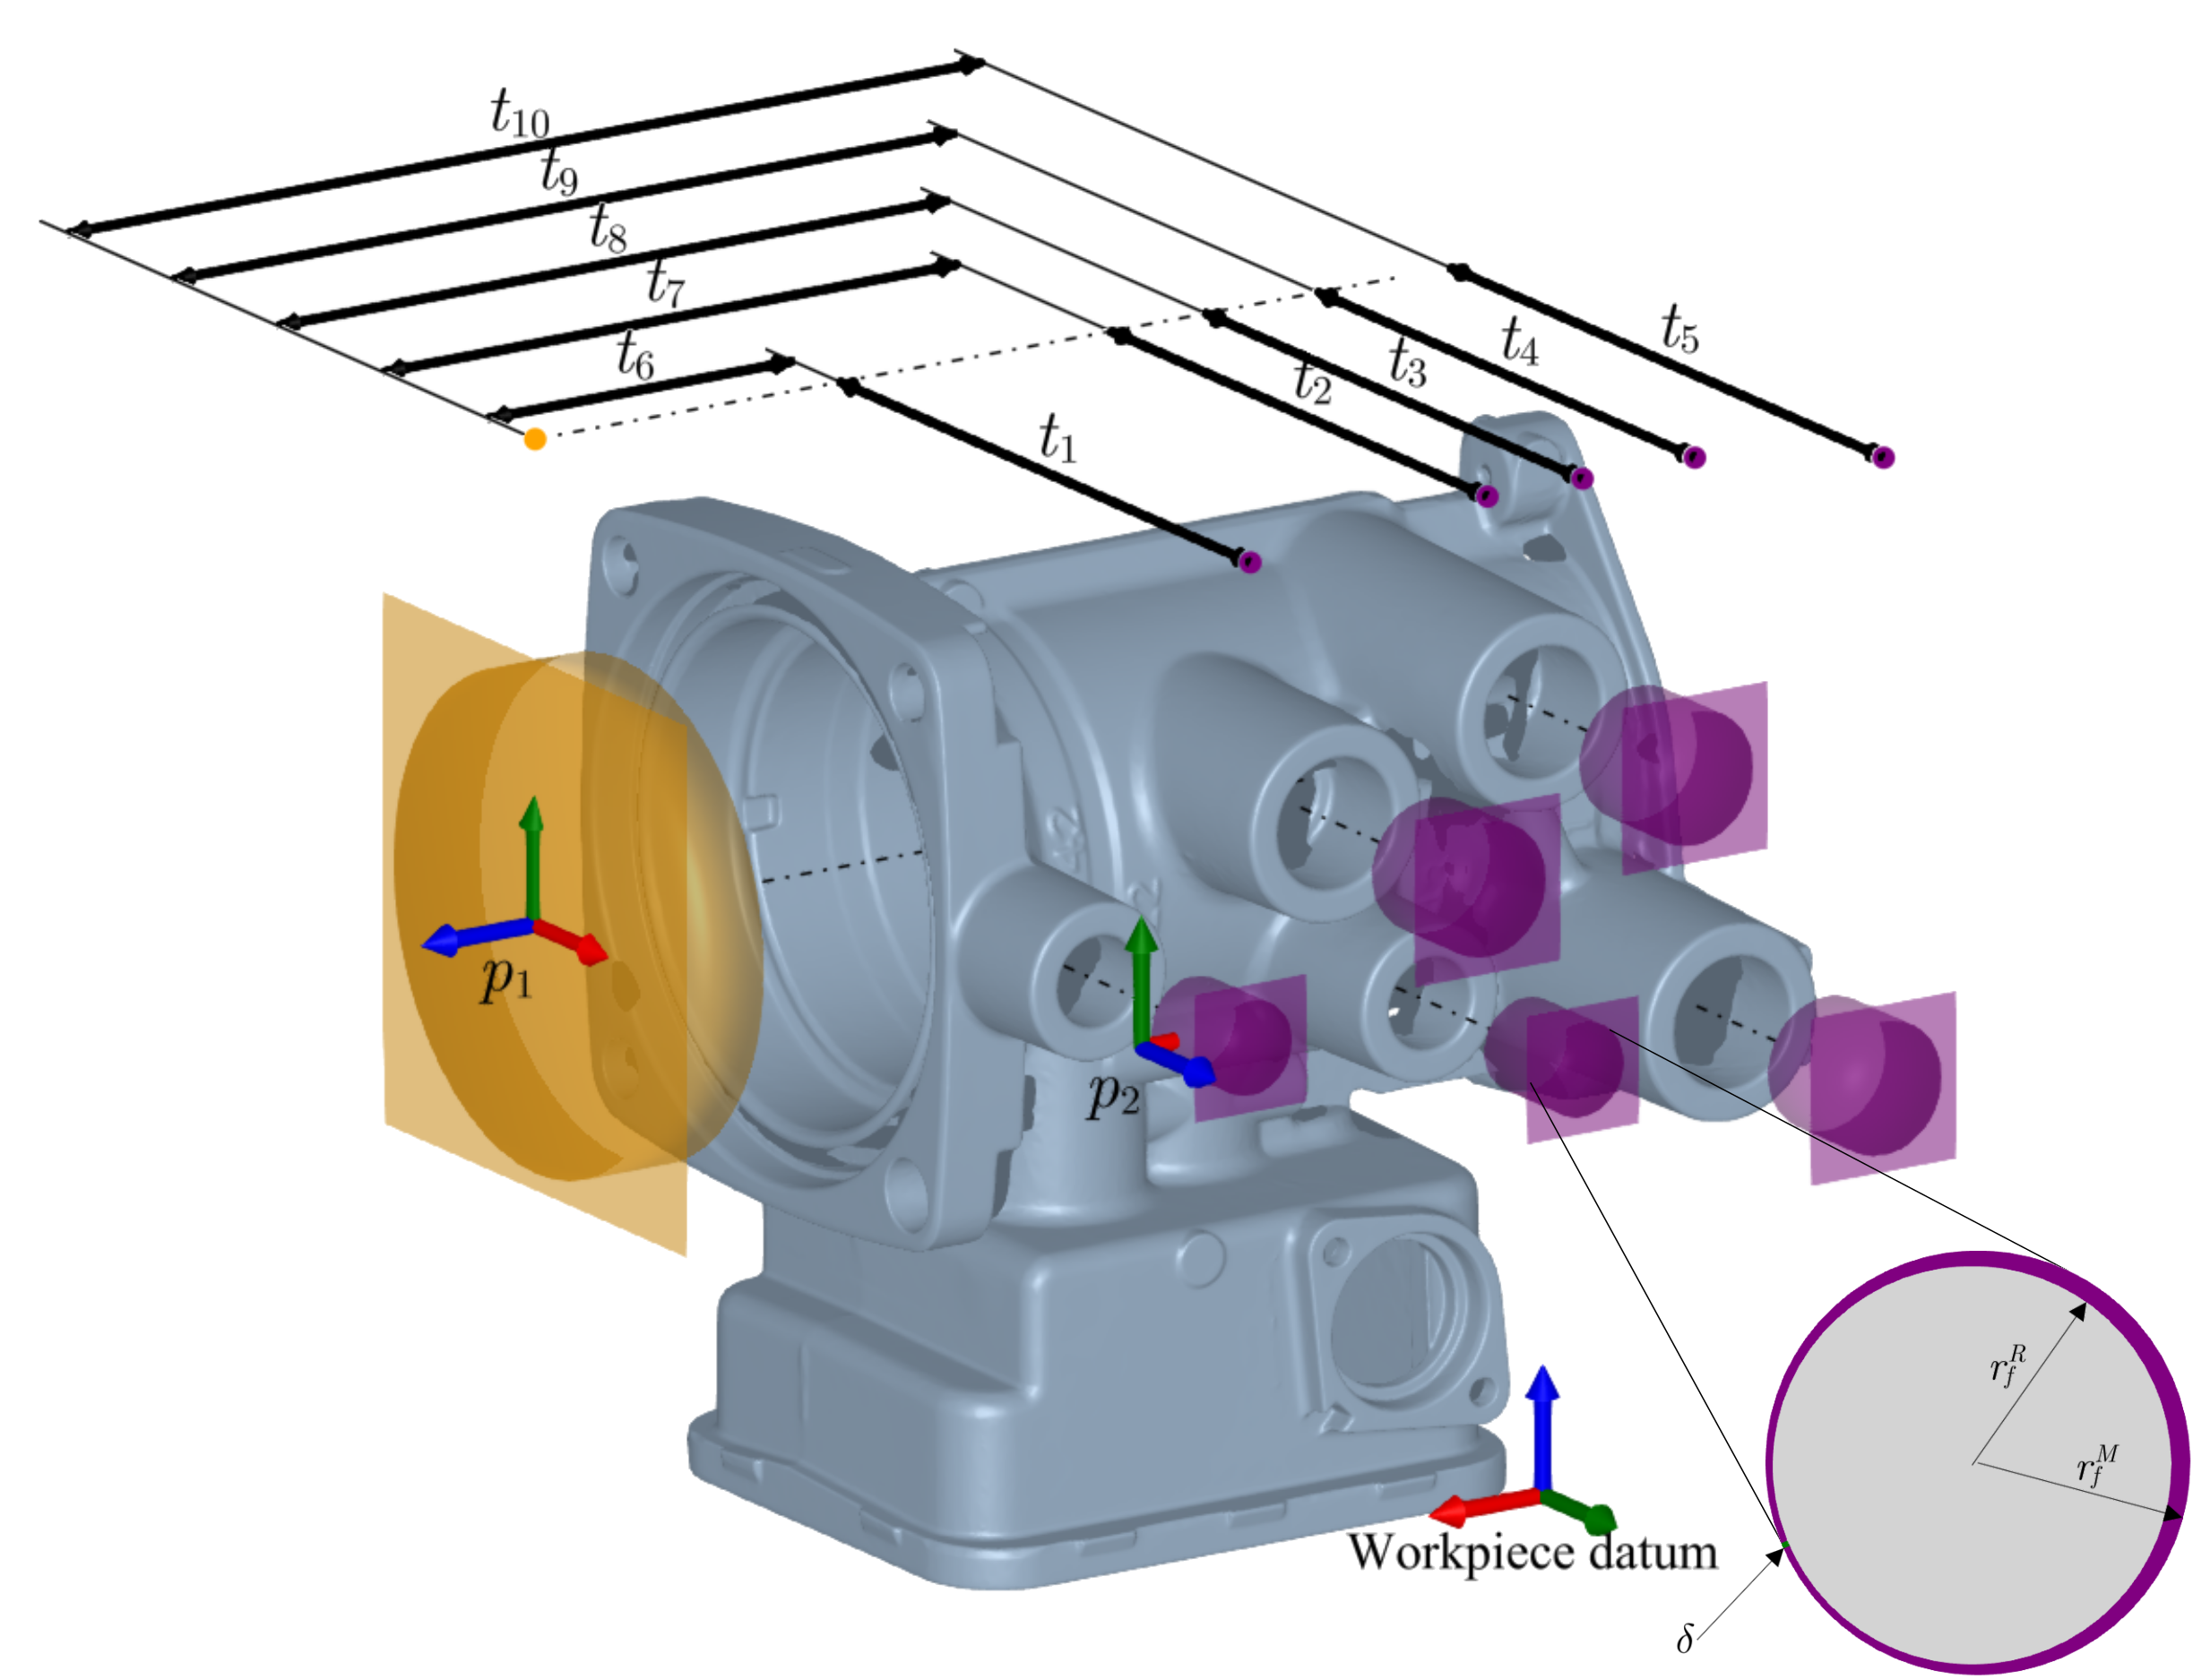
\includegraphics[width=0.95\columnwidth]{cirp-annals-2023-figure-2.png}}
	\caption{Measured part with two machined feature groups and tolerances between them. $r^M$ and $r^R$ denote the machined and rough radii of a feature, while $\delta$ the machining allowance \cite{cserteg:2023_Annals}.}
	\label{fig:hatfig}
\end{figure}

Inputs of the algorithm are the measured geometry of the rough part, the machining CNC code for each feature (relative to the corresponding part zero), the tolerance ranges for the features, and the minimum machining allowance parameter.
The output is the optimal position of the part zeros, where optimal means the lowest average tolerance error subject to a given machining allowance.

Measurements of the rough parts can be obtained with a variety of instruments, including coordinate measurement machines (CMM), laser scanners, measurement arms, etc.
The two main representations that these devices create are primitive geometries (cylinders, planes, etc.) and free-form geometries in the form of point cloud or triangulated mesh.
These measurements are fed into the optimization model, which is a convex quadratically constrained quadratic program (QCQP).
Details of the optimization model can be found in the papers \cite{cserteg:2023_CMS} and \cite{cserteg:2023_Annals}.

\section{Implementation in Julia}
\label{sec:approach}

During the development of the algorithm, we needed an environment (package) that supports the quick prototyping needs of research, while giving a solid foundation to validate the concept with our industry partner as well.
These needs include:

\begin{itemize}
	\item A versatile type system for geometrical representation, especially regarding the differences of drilling/milling operations and free-form/primitive geometry representation.
	\item Easy-to-use interface for the optimization model.
	\item Support for importing geometries from a variety of measurement tools (CMM, laser scanner, measurement arm).
	\item Support for debugging, analyzing and visualizing the results.
\end{itemize}

A flexible type system is designed to handle the different representations of geometries and features.
Abstract hole and plane geometries model the drilling and milling operations, while traits describe if a feature uses a free-form or a primitive representation.
An internal API (set of functions) is designed to access the relevant properties of the geometries (center point, radius, surface points, etc.).

This internal API is used when constructing the optimization model utilizing the JuMP ecosystem~\cite{Lubin2023}.
With JuMP's excellent design, coding the optimization model was as easy as repeating the mathematical model in Julia.
Other advantage of the JuMP ecosystem is that solvers can be easily swapped if needed.
For development, the FICO Xpress solver was used (with academic license), but our industry partner could use the Ipopt or SCIP solvers without issue.
Using the internal API gives the advantage that new geometry representations can be quickly used with the optimization model by just implementing a new type and a set of functions.

As mentioned earlier, an important requirement was to handle the output formats of many different devices.
Every measurement instrument comes with its own processing software and export formats, not necessarily designed for interoperability.
As a result, we needed to write (or use) parsers for different text and tabular formats.

The geometric computations are implemented with the help of the \texttt{Meshes.jl} package, which enabled us to easily visualize the geometries and results from the beginnings, see Fig.~\ref{fig:hatfig} for an example.

\section{Results and future work}
\label{sec:results}

Fig.~\ref{fig:pareto} shows the allowance-tolerance pairs for an experiment from \cite{cserteg:2023_Annals}.
The diagram illustrates that the proposed algorithm (blue curve) leads to lower tolerance errors for any given machining allowance than earlier approaches, and it can also ensure significantly larger machining allowance.
Obviously, there is a trade-off between small tolerance error and large machining allowance.
Preliminary results were first published in \cite{cserteg:2023_DigitalTwinAssisted}.
A journal paper describes the original algorithm \cite{cserteg:2023_Annals}, and a conference paper details the modifications for free-form surfaces \cite{cserteg:2023_CMS}.

\begin{figure}[t]
	\centerline{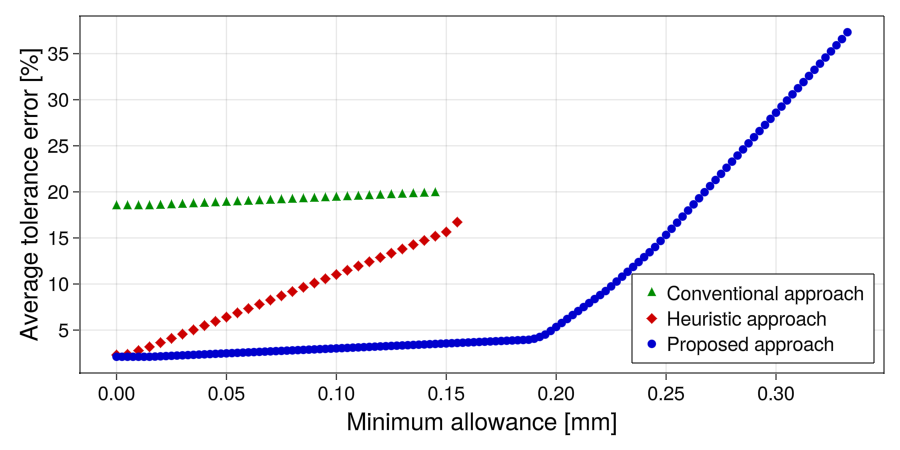
\includegraphics[width=0.95\columnwidth]{pareto-new-label.png}}
	\caption{Balancing the machining allowance and the tolerance error \cite{cserteg:2023_Annals}.}
	\label{fig:pareto}
\end{figure}

Future plans for the package and the method itself include an overhaul of the tolerance modeling scheme.
Currently, only dimensional tolerances are handled, but it should be discovered if more GD\&T tolerances can be incorporated into the model.
The current implementation supports only cylinders and planes, thus drilling and milling; it is a future research direction to extend the handled machining operations, e.g., to turning.

\section{Acknowledgments}
The research was supported by the European Union within the framework of the National Laboratory for Autonomous Systems (RRF-2.3.1-21-2022-00002) and the TKP2021-NKTA-01  NRDIO grant on "Research on cooperative production and logistics systems to support a competitive and sustainable economy".

% **************GENERATED FILE, DO NOT EDIT**************

\bibliographystyle{juliacon}
\bibliography{ref.bib}


\end{document}

% Inspired by the International Journal of Computer Applications template
